\section{Solutions to Protect against FIAs}

%%%%%%%%%%%%%%%%%%%%%%%%%%%%%%%%%%%%%%%%%%%%%%%%%%%%%%%%%%%%%%%%%%%%%%%%%%%%%%%%%%%%%%%%%%%%%%%%%%%%%%%%%%%%
\begin{frame}{Introduction}
    \begin{block}{Protections}
        \begin{itemize}
            \item Focusing on lightweight hardware countermeasures:
            \begin{itemize}
                \item \textbf{Hardware redundancy}: duplication, or triplication, of the circuit to compare the results obtained to check for any difference;
                \item \textbf{Temporal redundancy}: repeating operations in reverse to compare the result with the initial value;
                \item \textbf{Instruction replay}: executing multiple times the same instruction or block of instructions;
                \item \textbf{Obfuscation}: addition of dummy cycles, or shuffle the data;
                \only<1>{\item \textbf{Information redundancy}: adding additional data to the information to detect or correct the initial value, such as simple parity code, Hamming Code, BCH code, or Reed-Solomon.}
                \only<2>{\item \textcolor{red}{\textbf{Information redundancy}: adding additional data to the information to detect or correct the initial value, such as simple parity code, Hamming Code, BCH code, or Reed-Solomon.}}
            \end{itemize}
        \end{itemize}
    \end{block}

    \note{lightweight : only add a few bits of data without an overhead on performances to detect and correct 1 or 2 errors}
\end{frame}
%%%%%%%%%%%%%%%%%%%%%%%%%%%%%%%%%%%%%%%%%%%%%%%%%%%%%%%%%%%%%%%%%%%%%%%%%%%%%%%%%%%%%%%%%%%%%%%%%%%%%%%%%%%%
\begin{frame}{Countermeasures}
    \begin{block}{Protections}
        \begin{itemize}
            \item Focusing on information redundancy codes:
            \begin{itemize}
                \item Simple parity
                \item Hamming Code
                \item Hamming Code with an additional bit (SECDED)
            \end{itemize}
            \item Implementations of \textit{Hamming Code} and \textit{Simple parity} have been presented at ISVLSI 2024~\cite{PRLG-24-isvlsi}.
        \end{itemize}
    \end{block}
\end{frame}
%%%%%%%%%%%%%%%%%%%%%%%%%%%%%%%%%%%%%%%%%%%%%%%%%%%%%%%%%%%%%%%%%%%%%%%%%%%%%%%%%%%%%%%%%%%%%%%%%%%%%%%%%%%%
\subsection{Simple Parity}
    \begin{frame}{Detection of single-bit errors - Simple Parity}
        \begin{block}{}
            \begin{itemize}
                \justifying
                \item Often used for error detection.
                \item Add an extra bit for parity computation.
                \item Can only detect one error without correction.
            \end{itemize}
        \end{block}

        \vfill
        
        \begin{figure}
            \centering
            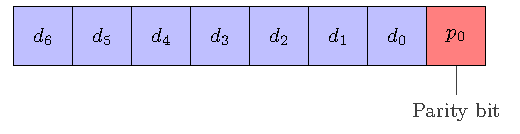
\includegraphics[width=.5\textwidth, page=1]{src/4_strategies/img/simple_parity.pdf}
            \caption{Simple parity codeword}
            \label{fig:simple_parity_codeword}
        \end{figure}
    \end{frame}
%%%%%%%%%%%%%%%%%%%%%%%%%%%%%%%%%%%%%%%%%%%%%%%%%%%%%%%%%%%%%%%%%%%%%%%%%%%%%%%%%%%%%%%%%%%%%%%%%%%%%%%%%%%%
\subsection{Hamming Code}
    \begin{frame}{Detection and correction of single-bit errors - Hamming Code}
        \begin{block}{}
            \begin{itemize}
                \justifying
                \item Linear error-correcting codes invented by Richard W. Hamming~\cite{H-50-bstj}.
                \item Mostly used in digital communication and data storage systems.
                \item Detect and correct single-bit error.
                \item Redundancy bits are placed in power of 2 positions.
                % \item The number of redundancy bits depends on the number of bits to be protected {\scriptsize ($ 2^r \ge m + r + 1 $)}
            \end{itemize}
        \end{block}

        \begin{minipage}[c]{0.4\linewidth}
            \begin{equation} \label{equat:hamming_encoder}
                \begin{split}
                    r_{0} &= d_{0} \oplus d_{1} \oplus d_{3} \oplus d_{4} \oplus d_{6} \\
                    r_{1} &= d_{0} \oplus d_{2} \oplus d_{3} \oplus d_{5} \oplus d_{6} \\
                    r_{2} &= d_{1} \oplus d_{2} \oplus d_{3} \\
                    r_{3} &= d_{4} \oplus d_{5} \oplus d_{6}
                \end{split}
            \end{equation}
        \end{minipage}\hfill%
        \begin{minipage}[c]{0.55\linewidth}
            \begin{figure}
                \centering
                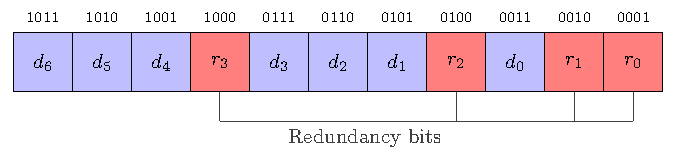
\includegraphics[width=\textwidth, page=1]{src/4_strategies/img/hamming_bit.pdf}
                \caption{Hamming codeword}
                \label{fig:hamming_codeword}
            \end{figure}
        \end{minipage}
    \end{frame}
%%%%%%%%%%%%%%%%%%%%%%%%%%%%%%%%%%%%%%%%%%%%%%%%%%%%%%%%%%%%%%%%%%%%%%%%%%%%%%%%%%%%%%%%%%%%%%%%%%%%%%%%%%%%
\subsection{Hamming Code - SECDED}
\begin{frame}{Detection of two-bit errors and correction of single-bit errors - SECDED}
    \begin{block}{}
        \begin{itemize}
            \justifying
            \item Based on Hamming Code.
            \item Detect two-bit error and correct single-bit error.
            \item An additional bit is added: general parity bit
        \end{itemize}
    \end{block}

    \begin{minipage}[c]{0.4\linewidth}
        \begin{equation} \label{equat:secded_encoder}
            \begin{split}
                r_{0}  &= d_{0} \oplus d_{1} \oplus d_{3} \oplus d_{4} \oplus d_{6} \\
                r_{1}  &= d_{0} \oplus d_{2} \oplus d_{3} \oplus d_{5} \oplus d_{6} \\
                r_{2}  &= d_{1} \oplus d_{2} \oplus d_{3} \\
                r_{3}  &= d_{4} \oplus d_{5} \oplus d_{6} \\
                gp_{0} &= \bigoplus_{i=0}^{6} d_{i} \oplus \bigoplus_{j=0}^{3} r_{j}
            \end{split}
        \end{equation}
    \end{minipage}\hfill%
    \begin{minipage}[c]{0.6\linewidth}
        \begin{figure}
            \centering
            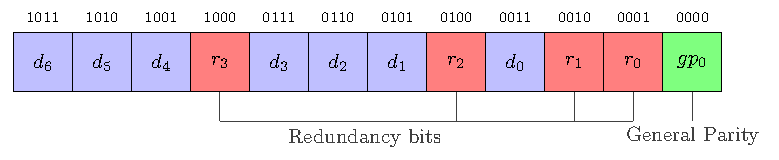
\includegraphics[width=\textwidth, page=1]{src/4_strategies/img/secded.pdf}
            \caption{SECDED codeword}
            \label{fig:secded_codeword}
        \end{figure}
    \end{minipage}
\end{frame}

\begin{frame}{Implementation - One register for one encoder}
    \begin{figure}
        \centering
        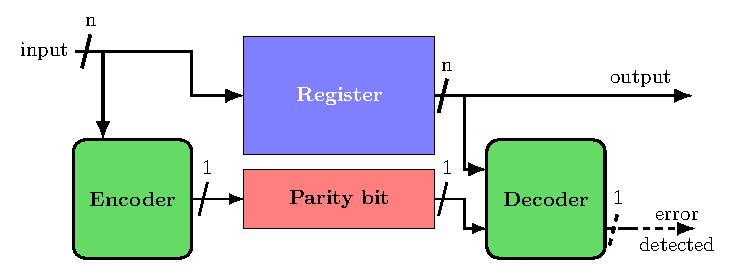
\includegraphics[width=.75\textwidth, page=1]{src/4_strategies/img/archi_contremesures.pdf}
        \caption{Implementation of a protection for one register}
        \label{fig:simple_parity_implem}
    \end{figure}
\end{frame}

\begin{frame}{Implementation - Multiple registers for one encoder}
    \begin{figure}
        \centering
        \includegraphics[width=.8\textwidth, page=4]{src/4_strategies/img/archi_contremesures.pdf}
        \caption{SImplementation of a protection for multiple registers}
        \label{fig:secded_implem_independant_register}
    \end{figure}
\end{frame}

\begin{frame}{Implementation - One register on multiple encoders}
    \begin{figure}
        \centering
        \includegraphics[width=.9\textwidth, page=6]{src/4_strategies/img/archi_contremesures.pdf}
        \caption{Implementation of a protection for one register splitted}
        \label{fig:secded_implem_splitted}
    \end{figure}
\end{frame}

\begin{frame}{Implementation - Special case for Register File tag}
    \begin{figure}
        \centering
        \includegraphics[width=.9\textwidth, page=5]{src/4_strategies/img/archi_contremesures.pdf}
        \caption{Special implementation for the Register File Tag}
        \label{fig:secded_implem_rf}
    \end{figure}
\end{frame}
%%%%%%%%%%%%%%%%%%%%%%%%%%%%%%%%%%%%%%%%%%%%%%%%%%%%%%%%%%%%%%%%%%%%%%%%%%%%%%%%%%%%%%%%%%%%%%%%%%%%%%%%%%%%
\begin{frame}{Implemented strategies - Evaluation of Group Composition}
    \begin{block}{}
        \begin{itemize}
            \justifying
            \item Different strategies of implementation can be done depending on the objective
            \item The protection efficiency would vary
            \item We want the best protection at the lowest cost possible against different fault models
        \end{itemize}
    \end{block}
\end{frame}

\begin{frame}{Implemented strategies - Group composition}
    \begin{table}[t]
        \centering
        \small
        \caption{Grouping composition and objectives of implemented strategies}
        \label{tab:strategies_group}
        % \setlength{\tabcolsep}{2pt}
        \begin{tabular}{@{}cm{4cm}m{7cm}@{}}
            \toprule
                                & \tableCentered{Grouping strategy}           & Objective                                                       \\ \midrule
            Strategy 1          & Minimisation of groups                      & Minimisation of the area overhead                               \\
            Strategy 2          & Protection per pipeline stage               & One protection for each 7 pipeline stages                       \\
            Strategy 3          & Protection per register                     & Each register is protected individually                         \\
            Strategy 4          & Protection per register with CSR splitting  & Strategy 3 + Split the CSRs registers by group of operations    \\
            Strategy 5          & Coupling split registers                    & Split each register and couple each bit to another register     \\
            \bottomrule
        \end{tabular}
    \end{table}
\end{frame}
%%%%%%%%%%%%%%%%%%%%%%%%%%%%%%%%%%%%%%%%%%%%%%%%%%%%%%%%%%%%%%%%%%%%%%%%%%%%%%%%%%%%%%%%%%%%%%%%%%%%%%%%%%%%
\begin{frame}{Implemented strategies - details}
    \begin{figure}
        \centering
        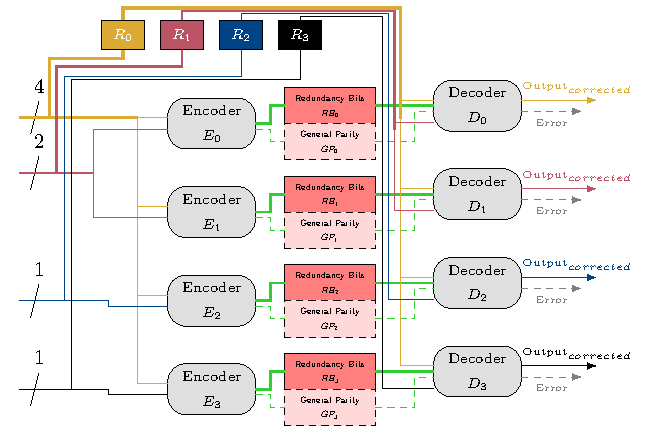
\includegraphics[height=.8\textheight]{src/4_strategies/img/implem5_spaghetti.pdf}
        \caption{Representation of the fifth strategy}
        \label{fig:strategy_5}
    \end{figure}
\end{frame}
%%%%%%%%%%%%%%%%%%%%%%%%%%%%%%%%%%%%%%%%%%%%%%%%%%%%%%%%%%%%%%%%%%%%%%%%%%%%%%%%%%%%%%%%%%%%%%%%%%%%%%%%%%%%